\documentclass[12pt, oneside]{book}   	% use "amsart" instead of "article" for AMSLaTeX format
\usepackage{geometry}                		% See geometry.pdf to learn the layout options. There are lots.
\geometry{a4paper}                   		% ... or a4paper or a5paper or ... 
%\geometry{landscape}                		% Activate for rotated page geometry
%\usepackage[parfill]{parskip}    		% Activate to begin paragraphs with an empty line rather than an indent
\usepackage{graphicx}				% Use pdf, png, jpg, or eps§ with pdflatex; use eps in DVI mode
								% TeX will automatically convert eps --> pdf in pdflatex		
\usepackage{amssymb}
\usepackage{fancyhdr}
\usepackage{color}
\usepackage[latin1]{inputenc}
\usepackage{amsmath}
%SetFonts

%SetFonts
\pagestyle{fancy}
\begin{document}
\thispagestyle{empty}
\hspace{10cm}
Release date 04-01-2015
\\
\\
\begin{center}
{\huge Software Engineering 2:}
{\huge MyTaxiService}
\end{center}
\vspace*{\fill}
\begin{center}
\textbf{\huge Inspection Document} 
\\
\large{V1.0}
\end{center}
\vfill
\begin{center}
{\large Dimitar Anastasovski, Marco Colombo}
\end{center}
\clearpage
\pagestyle{plain}
\tableofcontents
\setcounter{page}{1}
\clearpage
\chapter{Assigned classes}
We only have one class called \textbf{PolicyParser.java}
\newline
\newline
\textbf{\Large{Methods:}}
\newline
\begin{itemize}
\item{\textbf{Name:}getStorePassURL( )
\newline
\textbf{Start Line:}293
\newline
\textbf{Location:}appserver/security/core-ee/src/main/java/com/sun/enterprise
\newline
/security/provider/PolicyParser.java}
\newline
\item{\textbf{Name:}parseKeyStoreEntry( )
\newline
\textbf{Start Line:}358
\newline
\textbf{Location:}appserver/security/core-ee/src/main/java/com/sun/enterprise
\newline
/security/provider/PolicyParser.java}
\newline
\item{\textbf{Name:}writeKeyStoreEntry( PrintWriter out )
\newline
\textbf{Start Line:}397
\newline
\textbf{Location:}appserver/security/core-ee/src/main/java/com/sun/enterprise
\newline
/security/provider/PolicyParser.java}
\newline
\item{\textbf{Name:}parseGrantEntry( )
\newline
\textbf{Start Line:}420
\newline
\textbf{Location:}appserver/security/core-ee/src/main/java/com/sun/enterprise
\newline
/security/provider/PolicyParser.java}
\end{itemize}
\chapter{Functional role}
The policy for a Java runtime (specifying which permissions are available for code from various principals) is represented as a separate persistent configuration. The configuration may be stored as a flat ASCII file, as a serialized binary file of the Policy class, or as a database.
\newline
The Java runtime creates one global Policy object, which is used to represent the static policy configuration file. It is consulted by a ProtectionDomain when the protection domain initializes its set of permissions.
\newline
The Policy init method parses the policy configuration file, and then populates the Policy object. The Policy object is agnostic in that it is not involved in making policy decisions. It is merely the Java runtime representation of the persistent policy configuration file.
\newline
When a protection domain needs to initialize its set of permissions, it executes code such as the following to ask the global Policy object to populate a Permissions object with the appropriate permissions:
\newline

  \thinspace policy = Policy.getPolicy();
 \newline
 
  \thinspace Permissions perms = policy.getPermissions(protectiondomain)
 \newline
 \newline
The protection domain contains CodeSource object, which encapsulates its codebase (URL) and public key attributes. It also contains the principals associated with the domain. The Policy object evaluates the global policy in light of who the principal is and what the code source is and returns an appropriate Permissions object.
\clearpage
\textbf{\Large{Methods:}}
\begin{itemize}
\item getStorePassURL( )
\end{itemize}
\begin{figure}[h]
\center 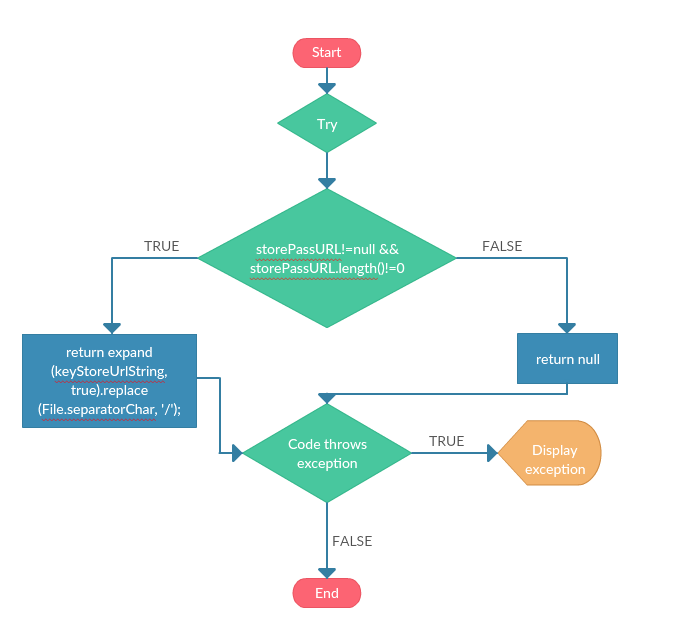
\includegraphics[scale=0.6]{getStorePassURL.png}
\end{figure}
\clearpage
\begin{itemize}
\item parseKeyStoreEntry( )
\end{itemize}
\begin{figure}[h]
\center 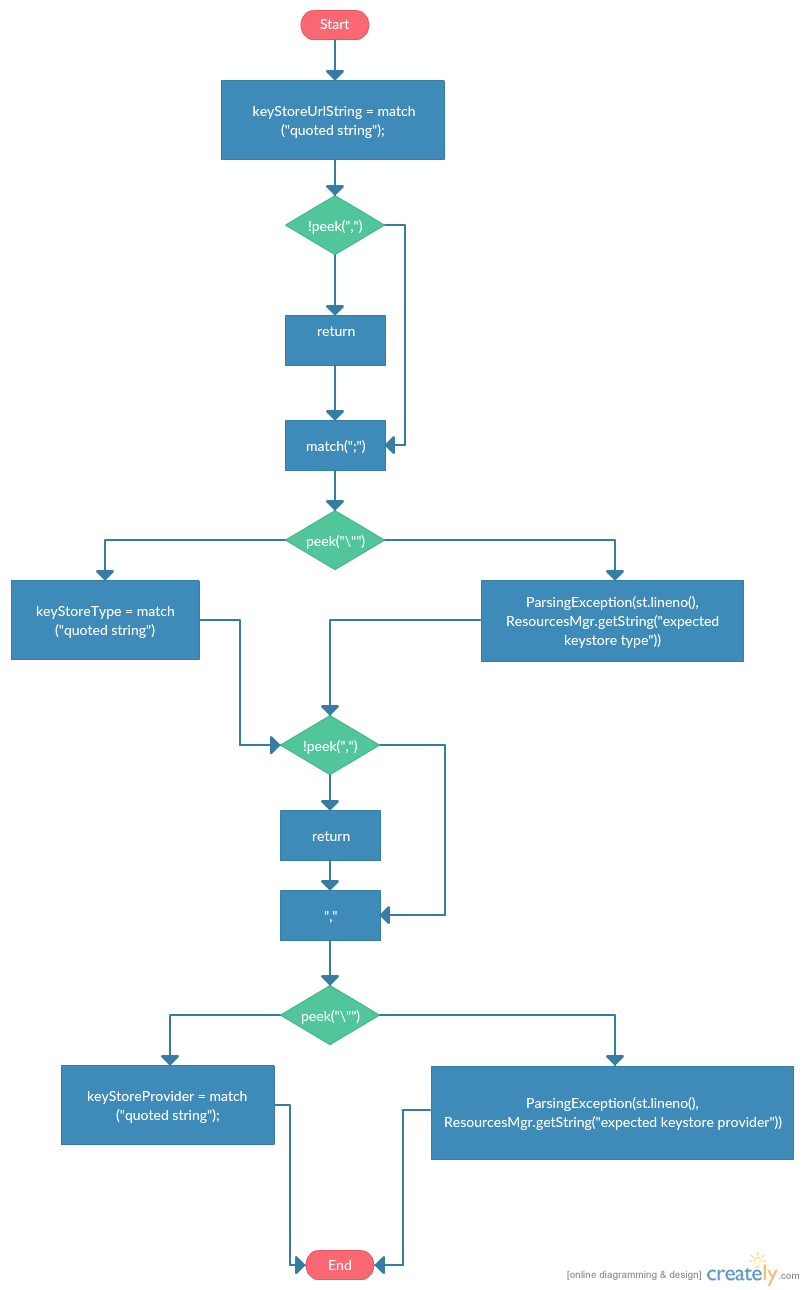
\includegraphics[scale=0.35]{parseKeyStoreEntry.jpg}
\end{figure}
\clearpage
\begin{itemize}
\item writeKeyStoreEntry(PrintWriter out)
\end{itemize}
\begin{figure}[h]
\center 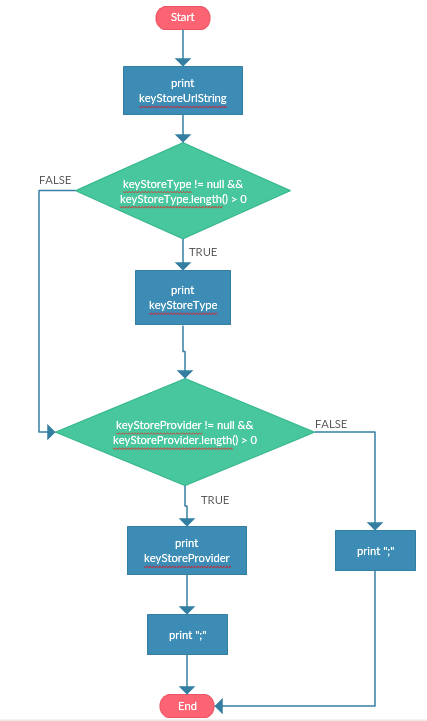
\includegraphics[scale=0.6]{writeKeyStoreEntry.png}
\end{figure}
\chapter{Issues}
\section{Naming Conventions}
No issues here
\section{Indention}
\begin{enumerate}
\item Line 432 more than 9 spaces applied
\newline  Line 444 more than 9 spaces applied
\item No issues
\end{enumerate}
\section{Braces}
Keringhan and Ritchie styke is used in whole class 
\section{Wrapping lines}
Line 355 line break not correct 
\newline
Line 364 line break not correct 
\newline
Line 443 line break not correct 
\newline
Line 463 line break not correct 
\section{File Organization}
No issues here
\section{Wrapping lines}
No issues here
\section{Comments}
Comments styles are different in the whole code. For example: 
\newline
\newline
// parse keystore type 
\newline
\newline
or
\newline
\newline
/**
\newline    
* parses a keystore entry
\newline 
*/
\section{Java Source File}
No issues here
\section{Package and import statements}
No issues here
\section{Class and interface declaration}
No issues here
\section{Initialization and Declarations}
No issues here
\section{Method Calls}
No issues here
\section{Arrays}
No issues here
\section{Object Comparison}
No issues here
\section{Output Format}
Line 410 output formal is not clear and formal
\section{Computation, Comparisons and Assignments}
Line 401,549,575 brutish programing is present
\section{Exceptions}
Line 542 exception is thrown but not catch properly in the function. 
\section{Flow of Control}
No issues here
\section{Files}
No issues here
\chapter{References}
\section{Software and used Tools}
\begin{itemize}
\item TexShop (http://pages.uoregon.edu/koch/texshop/), to redact this document
\end{itemize}
\section{Working hours}
\textbf{Dimitar Anastasovski:} $\thicksim$ hours
\\
\\
\textbf{Marco Colombo:} $\thicksim$ hours
\end{document}  